\chapter{Dynamic Programming}

So far in this book you have met two great strategies for designing
algorithms. Divide and conquer chops a problem into \emph{independent}
pieces, solves each, and glues the answers together. Greedy methods (which
get their own chapter next) make one locally best choice at a time and never
look back. Dynamic programming sits between them, and it is, honestly, one of
the most beautiful ideas in the whole subject. It is the technique you reach
for when a problem can be broken into subproblems, but the subproblems
\emph{overlap} -- the same little question gets asked again and again -- and
when the best overall answer is built out of best answers to those smaller
questions.

The name is historical and a little misleading; we will untangle it later.
For now, hold on to a single sentence: dynamic programming is the art of
\emph{not solving the same subproblem twice}. Everything else in this chapter
is a refinement of that sentence.

\begin{intuitionbox}
Imagine you are climbing a staircase and someone asks, ``how many distinct
ways can you reach step 30?'' You realize that the number of ways to reach
step 30 is just the number of ways to reach step 29 plus the number of ways
to reach step 28 (you arrive by a final hop of one or two). The same is true
for step 29, which leans on 28 and 27, and so on down. If you computed this by
blind recursion you would recompute the answer for step 25 thousands of times.
Dynamic programming says: compute the answer for each step \emph{once}, write
it in a little notebook, and look it up forever after. That notebook -- a
table of solved subproblems -- is the soul of the method.
\end{intuitionbox}

We will build the whole machine slowly, on four classic problems: cutting a
steel rod into pieces, multiplying a chain of matrices, finding the longest
common subsequence of two strings, and building an optimal binary search tree.
By the end you will recognize the shape of a dynamic-programming problem on
sight, and you will know the two mechanical ways to turn that recognition into
working code.

\section{A First Problem: Cutting a Rod}
\label{ch15:rod}

A company buys long steel rods and cuts them into shorter rods to sell. A rod
of integer length $n$ inches can be cut into pieces of integer lengths, and a
piece of length $i$ sells for a known price $p_i$. The prices are not
proportional to length -- there are wholesale and scarcity effects -- so a
short piece can be surprisingly valuable. The question is simple to state and
genuinely not obvious: \emph{given a rod of length $n$ and the price table,
what is the maximum revenue $r_n$ you can earn by cutting it up (or leaving it
whole)?}

Here is the price table we will use for the entire section.

\begin{center}
\begin{tabular}{l rrrrrrrrrr}
\toprule
length $i$ & 1 & 2 & 3 & 4 & 5 & 6 & 7 & 8 & 9 & 10 \\
price $p_i$ & 1 & 5 & 8 & 9 & 10 & 17 & 17 & 20 & 24 & 30 \\
\bottomrule
\end{tabular}
\end{center}

Let us warm up with tiny cases, by hand. A rod of length 1 can only be left
alone: $r_1 = 1$. A rod of length 2 can be left whole for $p_2 = 5$, or cut
into $1+1$ for $1+1 = 2$; the best is $r_2 = 5$. Length 3: whole gives $8$;
$1+2$ gives $1+5 = 6$; $1+1+1$ gives $3$. Best is $r_3 = 8$. Length 4 is the
first surprise: whole gives $p_4 = 9$, but $2+2$ gives $5+5 = 10$. So $r_4 =
10$, and the optimal solution is \emph{not} to leave it whole even though a
length-4 price exists. That is the whole reason the problem is interesting.

\subsection{Finding the recursive structure}

How would you reason about a rod of length $n$ in general? Picture making the
cuts left to right. Whatever the optimal cutting is, it begins with some
\emph{first} piece, of length $i$ for some $1 \le i \le n$. That first piece
earns exactly $p_i$. The rest of the rod, length $n-i$, is then a smaller copy
of \emph{the very same problem}: cut a rod of length $n-i$ for maximum
revenue. We do not know which first length $i$ is best, so we try them all and
keep the winner.

\begin{focusbox}
This gives the central recurrence for rod cutting:
\[
  r_n \;=\; \max_{1 \le i \le n}\bigl(\,p_i + r_{n-i}\,\bigr),
  \qquad r_0 = 0.
\]
In words: the best revenue for length $n$ equals the best, over all choices of
first-piece length $i$, of ``sell the first piece for $p_i$, then optimally cut
the remaining $n-i$ inches.'' The base case $r_0=0$ says an empty rod earns
nothing.
\end{focusbox}

This recurrence already exposes the two properties that make a problem suitable
for dynamic programming. The first we call \emph{optimal substructure}: the
optimal solution to the whole problem contains within it optimal solutions to
subproblems (the leftover rod is cut optimally, never wastefully). The second
is \emph{overlapping subproblems}: when you expand the recurrence you find that
$r_{n-i}$ for the same small value shows up over and over. We will make both
ideas precise in Section~\ref{ch15:elements}.

\subsection{The naive recursion and why it explodes}

If you translate the recurrence directly into code, you get this.

\begin{algorithm}[H]
\caption{\textsc{Cut-Rod}$(p, n)$ -- naive recursion}
\KwIn{price array $p[1\,..\,n]$, rod length $n$}
\KwOut{maximum revenue $r_n$}
\If{$n = 0$}{\Return $0$}
$q \gets -\infty$\;
\For{$i \gets 1$ \KwTo $n$}{
  $q \gets \max\bigl(q,\; p[i] + \textsc{Cut-Rod}(p, n-i)\bigr)$\;
}
\Return $q$\;
\end{algorithm}

This is correct, and for $n = 4$ it is fine. But watch what happens for larger
$n$. To solve length 4 we call lengths 3, 2, 1, 0. To solve length 3 we again
call 2, 1, 0. The same subproblems are re-solved in completely separate
branches of the recursion. The recursion tree below shows the calls for
$n = 4$; notice how often each node reappears.

\begin{center}
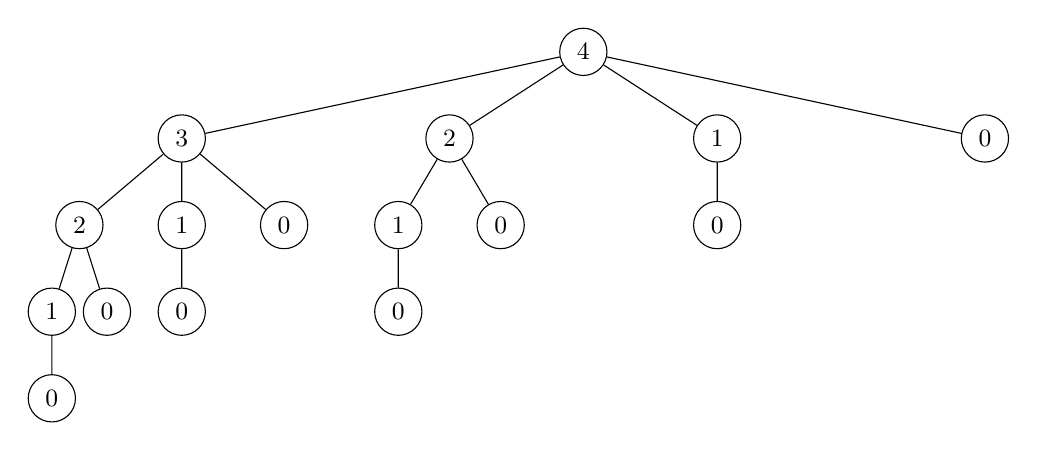
\begin{tikzpicture}[level distance=11mm,
  level 1/.style={sibling distance=34mm},
  level 2/.style={sibling distance=13mm},
  level 3/.style={sibling distance=7mm},
  every node/.style={draw,circle,inner sep=1pt,minimum size=6mm,font=\small}]
\node {4}
  child {node {3}
    child {node {2}
      child {node {1} child {node {0}}}
      child {node {0}}}
    child {node {1} child {node {0}}}
    child {node {0}}}
  child {node {2}
    child {node {1} child {node {0}}}
    child {node {0}}}
  child {node {1} child {node {0}}}
  child {node {0}};
\end{tikzpicture}
\end{center}

Let $T(n)$ count the number of calls \textsc{Cut-Rod} makes (including
itself) when solving length $n$. The root makes one call to itself plus one
call for each of $n-0, n-1, \dots, 1$, i.e.\ to lengths $0$ through $n-1$:
\[
  T(n) = 1 + \sum_{j=0}^{n-1} T(j), \qquad T(0) = 1.
\]
A little unrolling shows $T(n) = 2^n$. (Check: $T(0)=1$, $T(1)=1+T(0)=2$,
$T(2)=1+T(0)+T(1)=4$, $T(3)=8$.) The work doubles with every extra inch. That
is catastrophic -- length 40 would take a trillion calls -- and the cause is
pure waste: we keep re-deriving answers we already found.

\begin{trapbox}
A natural first reaction is ``this exponential blowup is fundamental to the
problem.'' It is not. The blowup is an artifact of the \emph{recursion}, not of
the \emph{problem}. There are only $n+1$ distinct subproblems ($r_0$ through
$r_n$). Any algorithm that solves each distinct subproblem once is already
polynomial. Dynamic programming is precisely the discipline of arranging that.
\end{trapbox}

\subsection{Memoization: the notebook fix}

The smallest possible change repairs the disaster. Keep an array $r[0\,..\,n]$,
initialized to ``unknown'' (we use $-\infty$ as a sentinel). Before solving a
subproblem, check the array; if the answer is already there, return it. After
solving it, store it. This top-down caching is called \emph{memoization}
(yes, no ``r'' -- as in writing a \emph{memo}).

\begin{algorithm}[H]
\caption{\textsc{Memoized-Cut-Rod}$(p, n)$}
\KwIn{price array $p[1\,..\,n]$, length $n$}
\KwOut{maximum revenue $r_n$}
let $r[0\,..\,n]$ be a new array, all entries $\gets -\infty$\;
\Return \textsc{MCR-Aux}$(p, n, r)$\;
\BlankLine
\textbf{procedure} \textsc{MCR-Aux}$(p, n, r)$\;
\If{$r[n] \ge 0$}{\Return $r[n]$ \tcp*{already solved}}
\eIf{$n = 0$}{$q \gets 0$}{
  $q \gets -\infty$\;
  \For{$i \gets 1$ \KwTo $n$}{
    $q \gets \max\bigl(q,\; p[i] + \textsc{MCR-Aux}(p, n-i, r)\bigr)$\;
  }
}
$r[n] \gets q$\;
\Return $q$\;
\end{algorithm}

Now each subproblem is genuinely solved once; subsequent requests are
one-line lookups. There are $n+1$ subproblems, and solving subproblem $j$ does
$O(j)$ work in its loop, so the total is $\sum_{j=0}^{n} O(j) = O(n^2)$. We
went from $2^n$ to $n^2$ by adding one array and one early-return.

The picture below makes the saving visible. On the left is the exploding
recursion tree of the naive call; on the right is what memoization (or
tabulation) actually computes -- the \emph{subproblem graph}, with one node per
distinct length and an edge $j \to j'$ whenever solving $j$ consults $j'$.
The tree has $2^n$ nodes; the graph has only $n+1$.

\begin{center}
\begin{tikzpicture}[every node/.style={draw,circle,inner sep=1pt,minimum size=6mm,font=\small}]
% subproblem DAG for n=4
\node (n0) at (0,0) {0};
\node (n1) at (1.7,0) {1};
\node (n2) at (3.4,0) {2};
\node (n3) at (5.1,0) {3};
\node (n4) at (6.8,0) {4};
\begin{scope}[-{Stealth[length=2mm]},sourceblue,thick]
\draw (n1) -- (n0);
\draw (n2) to[bend left=35] (n0);
\draw (n2) -- (n1);
\draw (n3) to[bend left=42] (n0);
\draw (n3) to[bend left=30] (n1);
\draw (n3) -- (n2);
\draw (n4) to[bend right=42] (n0);
\draw (n4) to[bend right=30] (n1);
\draw (n4) to[bend right=20] (n2);
\draw (n4) -- (n3);
\end{scope}
\end{tikzpicture}
\\[1mm]
{\small The subproblem graph for $n=4$: five nodes, a handful of edges. Each
node is solved once. Compare the $16$-node recursion tree above.}
\end{center}

\subsection{Tabulation: filling the table bottom-up}

There is a second, often tidier way to get the same effect. Instead of
recursing top-down and caching, go \emph{bottom-up}: solve the smallest
subproblem first, then the next, building up. This is called \emph{tabulation}.
For rod cutting, solve $r_0$, then $r_1$, then $r_2$, and so on; by the time you
reach $r_n$ every value you need is already sitting in the table.

\begin{algorithm}[H]
\caption{\textsc{Bottom-Up-Cut-Rod}$(p, n)$}
\KwIn{price array $p[1\,..\,n]$, length $n$}
\KwOut{maximum revenue $r_n$}
let $r[0\,..\,n]$ be a new array\;
$r[0] \gets 0$\;
\For{$j \gets 1$ \KwTo $n$}{
  $q \gets -\infty$\;
  \For{$i \gets 1$ \KwTo $j$}{
    $q \gets \max\bigl(q,\; p[i] + r[j-i]\bigr)$\;
  }
  $r[j] \gets q$\;
}
\Return $r[n]$\;
\end{algorithm}

The two nested loops make the $O(n^2)$ cost transparent: the inner loop runs
$j$ times for each $j$, and $\sum_{j=1}^n j = \tfrac{n(n+1)}{2} = \Theta(n^2)$.

\begin{labbox}
Let us run \textsc{Bottom-Up-Cut-Rod} on the price table, by hand, for $n=8$.
We fill $r[0]$ through $r[8]$, each time trying every first-piece length $i$
from $1$ to $j$ and recording the best $p_i + r[j-i]$.

\begin{center}
\begin{tabular}{c l c c}
\toprule
$j$ & best split tried & value & $r[j]$ \\
\midrule
0 & --- & --- & 0 \\
1 & $p_1+r_0=1+0$ & 1 & 1 \\
2 & $p_2+r_0=5+0$ & 5 & 5 \\
3 & $p_3+r_0=8+0$ & 8 & 8 \\
4 & $p_2+r_2=5+5$ & 10 & 10 \\
5 & $p_2+r_3=5+8$ & 13 & 13 \\
6 & $p_6+r_0=17+0$ & 17 & 17 \\
7 & $p_1+r_6=1+17$ \;or\; $p_6+r_1=17+1$ & 18 & 18 \\
8 & $p_2+r_6=5+17$ & 22 & 22 \\
\bottomrule
\end{tabular}
\end{center}

Trace $j=7$ carefully, since it has a tie. We try
$p_1+r_6=18$, $p_2+r_5=5+13=18$, $p_3+r_4=8+10=18$, $p_4+r_3=9+8=17$,
$p_5+r_2=10+5=15$, $p_6+r_1=17+1=18$, $p_7+r_0=17$. The maximum is $18$, and
several splits achieve it. The table does not care which -- it stores only the
value $18$. Reconstructing \emph{a} set of cuts is the next subsection.
\end{labbox}

\subsection{Reconstructing the actual cuts}

The table gives you the best \emph{revenue}, but a customer wants to know
\emph{where to cut}. The standard trick is to record, alongside each $r[j]$, the
first-piece length that achieved the maximum. We store it in a second array
$s[j]$.

\begin{algorithm}[H]
\caption{\textsc{Extended-Bottom-Up-Cut-Rod}$(p, n)$}
\KwIn{price array $p[1\,..\,n]$, length $n$}
\KwOut{revenue array $r$ and choice array $s$}
let $r[0\,..\,n]$ and $s[1\,..\,n]$ be new arrays; \quad $r[0]\gets 0$\;
\For{$j \gets 1$ \KwTo $n$}{
  $q \gets -\infty$\;
  \For{$i \gets 1$ \KwTo $j$}{
    \If{$q < p[i] + r[j-i]$}{
      $q \gets p[i] + r[j-i]$\;
      $s[j] \gets i$\;
    }
  }
  $r[j] \gets q$\;
}
\Return $(r, s)$\;
\end{algorithm}

To print the cuts for a rod of length $n$, peel off $s[n]$, then recurse on the
remainder $n - s[n]$:

\begin{algorithm}[H]
\caption{\textsc{Print-Cut-Rod-Solution}$(p, n)$}
let $(r,s) \gets$ \textsc{Extended-Bottom-Up-Cut-Rod}$(p,n)$\;
\While{$n > 0$}{
  print $s[n]$\;
  $n \gets n - s[n]$\;
}
\end{algorithm}

For our table, $s$ comes out as $s = [1,2,3,2,2,6,1,2]$ for $j=1..8$. For
$n=8$: $s[8]=2$, print $2$, go to $6$; $s[6]=6$, print $6$, go to $0$. So the
cut list is $2+6$, earning $5+17=22$. Confirmed against the table.

\begin{aestheticbox}
Rod cutting is a toy, but its skeleton -- ``the best first move plus the best
solution to what remains'' -- is exactly the structure of resource-allocation
problems that run the world: how to slice a fixed advertising budget across
channels, how to pack a knapsack of cargo, how to break a paragraph into lines
of justified text (the algorithm behind \TeX's beautiful line breaking is
dynamic programming), and how to schedule jobs for maximum profit. Learn the
skeleton once and you see it everywhere.
\end{aestheticbox}

\section{The Elements of Dynamic Programming}
\label{ch15:elements}

Step back. We solved one problem; now let us name the parts so we can find them
in the next problem fast. Every dynamic-programming algorithm is built from the
same four moving pieces.

\begin{focusbox}
The four-step recipe for designing a DP:
\begin{enumerate}
  \item \textbf{Characterize the structure} of an optimal solution: what is the
  ``last choice'' that splits a problem into subproblems?
  \item \textbf{Define the value} of an optimal solution recursively (write the
  recurrence, including base cases).
  \item \textbf{Compute that value}, usually bottom-up into a table (or
  top-down with memoization).
  \item \textbf{Reconstruct} an optimal solution from recorded choices (only if
  you need the solution itself, not just its value).
\end{enumerate}
\end{focusbox}

For step~3 to be possible at all, the problem must have two properties. They
are the litmus test for ``can I use DP here?''

\subsection{Optimal substructure}

\begin{definition}[Optimal substructure]
\label{ch15:def-optsub}
A problem has \emph{optimal substructure} if an optimal solution to the problem
contains within it optimal solutions to subproblems.
\end{definition}

In rod cutting, once you commit to a first piece of length $i$, the rest of the
rod \emph{must} be cut optimally -- if it were not, you could replace that part
with a better cutting and improve the whole, contradicting optimality. This
cut-and-paste argument is how you prove optimal substructure in general:
\emph{assume} the subpart is suboptimal, \emph{paste} in a better subpart, and
derive a better global solution than the supposedly optimal one. A
contradiction means the subpart was optimal all along.

\begin{trapbox}
Not every problem has optimal substructure, and the failures are instructive.
Consider \emph{unweighted longest simple path} in a graph. A longest simple
path from $u$ to $v$ need not decompose into a longest simple path from $u$ to
some intermediate $w$ plus one from $w$ to $v$ -- stitching two longest paths
can revisit a vertex and break simplicity. (Shortest paths, by contrast, do
have optimal substructure, which is why Dijkstra and friends exist.) Always
\emph{check} the property; do not assume it.
\end{trapbox}

\subsection{Overlapping subproblems}

\begin{definition}[Overlapping subproblems]
\label{ch15:def-overlap}
A problem has \emph{overlapping subproblems} if a recursive solution revisits
the same subproblem repeatedly, rather than always generating fresh ones.
\end{definition}

This is what divide-and-conquer problems usually \emph{lack}: when you split an
array for merge sort, the left and right halves are disjoint and never share
sub-instances, so caching buys nothing. Dynamic programming pays off precisely
when the subproblem space is small but the recursion keeps wandering back into
it. For rod cutting the space had size $n+1$ yet the naive recursion made $2^n$
calls; that gap of ``few distinct subproblems, many repeated visits'' is the
signature you are hunting for.

\begin{intuitionbox}
A clean way to see whether DP applies: draw the \emph{subproblem graph}. Put one
node per distinct subproblem, and an edge from $A$ to $B$ if solving $A$
directly needs the answer to $B$. For rod cutting this is a little chain
$r_n \to r_{n-1} \to \cdots \to r_0$ with extra forward edges. The number of
nodes is the number of distinct subproblems; the number of edges bounds the
total work. Bottom-up tabulation is just a topological-order sweep of this
graph. Memoization is a depth-first traversal that caches. If the graph is
small and acyclic, you win.
\end{intuitionbox}

\subsection{Memoization versus tabulation}

We have now seen both implementation styles. They compute the same answers and
have the same asymptotic cost; the choice is about taste and a few practical
trade-offs.

\begin{center}
\begin{tabular}{p{0.30\linewidth} p{0.30\linewidth} p{0.30\linewidth}}
\toprule
 & \textbf{Memoization (top-down)} & \textbf{Tabulation (bottom-up)} \\
\midrule
Control flow & recursion + cache & loops fill a table \\
Order solved & on demand, lazily & every subproblem, in order \\
Skips unused subproblems & yes & no (unless you are clever) \\
Recursion overhead & yes (stack frames) & none \\
Easy to add ``window'' space saving & harder & easier \\
Best when & subproblem space sparse, or recurrence awkward & all subproblems needed, order clear \\
\bottomrule
\end{tabular}
\end{center}

\begin{focusbox}
A useful default: \emph{think} with the top-down recurrence (it mirrors how you
reason), then \emph{write} bottom-up tabulation when every subproblem is needed
(it is faster and avoids deep recursion). Reach for memoization when only a
sparse slice of the table is actually visited, or when figuring out the correct
bottom-up filling order is genuinely fiddly.
\end{focusbox}

\begin{historybox}
The term ``dynamic programming'' was coined by Richard Bellman in the 1950s at
RAND. ``Programming'' meant planning/tabulation (as in ``linear programming''),
not coding; ``dynamic'' was chosen, by Bellman's own amused account, partly
because it sounded impressive and was hard for a budget-skeptical Secretary of
Defense to object to. The underlying idea -- Bellman's \emph{principle of
optimality} -- is exactly our optimal substructure. This chapter maps to CLRS
Chapter~15 in the 3rd edition and Chapter~14 in the 4th edition; the rod-cutting
opener, matrix-chain, LCS, and optimal BST examples all follow CLRS, which you
should read next for the rigorous treatment and additional problems.
\end{historybox}

\section{Matrix-Chain Multiplication}
\label{ch15:matrixchain}

Here is a problem where the DP is not over ``length'' but over
\emph{parenthesizations}, and it shows off optimal substructure beautifully.

You are given a chain of matrices $A_1, A_2, \dots, A_n$ to multiply together.
Matrix multiplication is associative -- you may group the product any way you
like and get the same matrix -- but the \emph{cost} of computing it depends
enormously on the grouping. Multiplying a $p \times q$ matrix by a $q \times r$
matrix using the standard algorithm costs $p \cdot q \cdot r$ scalar
multiplications. So the question is: \emph{how should you parenthesize the
chain to minimize the total number of scalar multiplications?}

\begin{example}[Why grouping matters]
\label{ch15:mc-example}
Take three matrices with dimensions $A_1: 10\times 100$, $A_2: 100\times 5$,
$A_3: 5\times 50$. Two groupings:
\[
  ((A_1 A_2) A_3):\quad 10\cdot 100\cdot 5 + 10\cdot 5\cdot 50 = 5000 + 2500 = 7500,
\]
\[
  (A_1 (A_2 A_3)):\quad 100\cdot 5\cdot 50 + 10\cdot 100\cdot 50 = 25000 + 50000 = 75000.
\]
Same answer matrix, but one grouping is \emph{ten times} cheaper. With a long
chain the gap can be astronomical.
\end{example}

We describe the chain by its dimension sequence $p_0, p_1, \dots, p_n$, where
matrix $A_k$ has dimensions $p_{k-1} \times p_k$. (Consecutive matrices share a
dimension, which is what makes them multipliable.) In the example,
$p = \langle 10, 100, 5, 50 \rangle$.

\subsection{The recurrence}

What is the ``last choice'' here? Any full parenthesization of
$A_i \cdots A_j$ splits, at the very top level, into a left group
$A_i \cdots A_k$ and a right group $A_{k+1} \cdots A_j$ for some split point
$k$ with $i \le k < j$. The two groups produce a $p_{i-1}\times p_k$ matrix and
a $p_k \times p_j$ matrix, and the final multiply costs
$p_{i-1}\,p_k\,p_j$. Let $m[i,j]$ be the minimum number of scalar
multiplications to compute $A_i \cdots A_j$. Then:

\begin{focusbox}
\[
  m[i,j] =
  \begin{cases}
    0 & \text{if } i = j,\\[4pt]
    \displaystyle \min_{i \le k < j}\Bigl(\, m[i,k] + m[k+1,j] + p_{i-1}\,p_k\,p_j \,\Bigr) & \text{if } i < j.
  \end{cases}
\]
A single matrix costs nothing. Otherwise, try every split point $k$, pay for
the best way to build each side plus the cost of the final multiply, and keep
the minimum.
\end{focusbox}

Optimal substructure: if the optimal parenthesization splits at $k$, then its
left subchain must itself be optimally parenthesized (cut-and-paste again: a
cheaper left grouping would cheapen the whole, contradiction). And the
subproblems overlap massively -- $m[2,4]$, say, is needed by many different
larger chains.

How many distinct subproblems are there? One for each pair $i \le j$, which is
$\binom{n}{2} + n = \Theta(n^2)$. Solving each tries up to $n$ split points, so
the total is $\Theta(n^3)$. (For comparison, the number of distinct
parenthesizations is the Catalan number, which grows like $4^n/n^{1.5}$ -- so
brute force is hopeless, and DP turns it polynomial.)

\subsection{Filling the table by chain length}

The base cases ($i=j$) sit on the diagonal of the table. Each $m[i,j]$ depends
on entries with \emph{shorter} chains ($m[i,k]$ and $m[k+1,j]$ each span fewer
matrices). So the safe filling order is by increasing chain length
$\ell = j - i + 1$, from $2$ up to $n$.

Geometrically, we fill the upper-triangular table one \emph{diagonal} at a time,
starting from the main diagonal of zeros and moving toward the lone top-right
corner that holds the final answer. The diagram shows the order for $n=6$: the
shaded cell $m[i,j]$ pulls from the row to its left ($m[i,k]$) and the column
below it ($m[k+1,j]$), both of which lie on already-completed diagonals.

\begin{center}
\begin{tikzpicture}[scale=0.72,every node/.style={font=\small}]
% grid for upper triangle, i rows 1..6 top to bottom, j cols 1..6 left to right
\foreach \i in {1,...,6}{
  \foreach \j in {1,...,6}{
    \ifnum\j<\i\relax\else
      \draw (\j-1,-\i+1) rectangle (\j,-\i);
    \fi
  }
}
% diagonal numbering (ell): cell (i,j) has ell=j-i+1; label a few diagonals
\foreach \i in {1,...,6}{ \node at (\i-0.5,-\i+0.5) {$0$}; }
% highlight target m[2,5] (i=2,j=5)
\fill[targetgreen!25] (4,-1) rectangle (5,-2);
\node at (4.5,-1.5) {$m_{2,5}$};
% dependency row cells m[2,k] k=2,3,4 and column cells m[k+1,5]
\foreach \k in {2,3,4}{ \fill[sourceblue!20] (\k-1,-1) rectangle (\k,-2); }
\fill[quotientorange!25] (4,-2) rectangle (5,-3); % m[3,5]
\fill[quotientorange!25] (4,-3) rectangle (5,-4); % m[4,5]
\fill[quotientorange!25] (4,-4) rectangle (5,-5); % m[5,5]
% redraw target on top
\fill[targetgreen!35] (4,-1) rectangle (5,-2);
\node at (4.5,-1.5) {$m_{2,5}$};
% top labels j
\foreach \j in {1,...,6}{ \node at (\j-0.5,0.35) {$j{=}\j$}; }
% left labels i
\foreach \i in {1,...,6}{ \node at (-0.6,-\i+0.5) {$i{=}\i$}; }
\end{tikzpicture}
\\[1mm]
{\small Computing $m_{2,5}$ (green): the minimum scans split points $k=2,3,4$,
each combining a blue cell from row $2$ ($m_{2,k}$) with an orange cell from
column $5$ ($m_{k+1,5}$). Both lie on shorter-chain diagonals, hence already
known.}
\end{center}

\begin{algorithm}[H]
\caption{\textsc{Matrix-Chain-Order}$(p)$}
\KwIn{dimension sequence $p[0\,..\,n]$ (so there are $n$ matrices)}
\KwOut{cost table $m$ and split table $s$}
\For{$i \gets 1$ \KwTo $n$}{$m[i,i] \gets 0$}
\For{$\ell \gets 2$ \KwTo $n$}{
  \For{$i \gets 1$ \KwTo $n-\ell+1$}{
    $j \gets i + \ell - 1$\;
    $m[i,j] \gets \infty$\;
    \For{$k \gets i$ \KwTo $j-1$}{
      $q \gets m[i,k] + m[k+1,j] + p[i-1]\cdot p[k]\cdot p[j]$\;
      \If{$q < m[i,j]$}{
        $m[i,j] \gets q$\;
        $s[i,j] \gets k$\;
      }
    }
  }
}
\Return $(m, s)$\;
\end{algorithm}

The three nested loops each run $O(n)$ times, giving $O(n^3)$ time, and the two
tables use $\Theta(n^2)$ space.

\begin{labbox}
Let us trace a real chain of six matrices, the classic CLRS instance, with
\[
  p = \langle 30,\ 35,\ 15,\ 5,\ 10,\ 20,\ 25 \rangle,
\]
so $A_1:30\times35$, $A_2:35\times15$, $A_3:15\times5$, $A_4:5\times10$,
$A_5:10\times20$, $A_6:20\times25$. We fill $m[i,j]$ diagonal by diagonal.

\textbf{Length 1} (the diagonal): all $m[i,i] = 0$.

\textbf{Length 2}: each is a single multiply.
\begin{align*}
m[1,2] &= p_0 p_1 p_2 = 30\cdot35\cdot15 = 15750,\\
m[2,3] &= 35\cdot15\cdot5 = 2625,\\
m[3,4] &= 15\cdot5\cdot10 = 750,\\
m[4,5] &= 5\cdot10\cdot20 = 1000,\\
m[5,6] &= 10\cdot20\cdot25 = 5000.
\end{align*}

\textbf{Length 3}: try both split points. For $m[1,3]$:
$k{=}1$ gives $0 + 2625 + 30\cdot35\cdot5 = 2625+5250 = 7875$;
$k{=}2$ gives $15750 + 0 + 30\cdot15\cdot5 = 15750+2250=18000$.
Minimum $7875$ at $k{=}1$.
Working out the rest of this diagonal the same way gives
$m[2,4]=4375$ ($k{=}3$), $m[3,5]=2500$ ($k{=}3$), $m[4,6]=3500$ ($k{=}5$).

\textbf{Length 4 and up}: continuing the sweep produces
$m[1,4]=9375$, $m[2,5]=7125$, $m[3,6]=5375$, then
$m[1,5]=11875$, $m[2,6]=10500$, and finally the answer $m[1,6]=15125$.
The full lower-triangular table:
\begin{center}
\begin{tabular}{c|cccccc}
 & $j{=}1$ & 2 & 3 & 4 & 5 & 6 \\
\hline
$i{=}1$ & 0 & 15750 & 7875 & 9375 & 11875 & \textbf{15125} \\
2 & & 0 & 2625 & 4375 & 7125 & 10500 \\
3 & & & 0 & 750 & 2500 & 5375 \\
4 & & & & 0 & 1000 & 3500 \\
5 & & & & & 0 & 5000 \\
6 & & & & & & 0 \\
\end{tabular}
\end{center}
The optimal cost is $m[1,6] = 15125$ scalar multiplications.
\end{labbox}

\subsection{Reconstructing the parenthesization}

The split table $s[i,j]$ records the best top-level split for each subchain. For
the trace above, $s[1,6] = 3$, meaning the best top split of $A_1\cdots A_6$ is
$(A_1 A_2 A_3)(A_4 A_5 A_6)$. Recursing with $s$ inside each side
($s[1,3]=1$, $s[4,6]=5$) yields the full grouping
\[
  \bigl((A_1 (A_2 A_3))\,((A_4 A_5) A_6)\bigr).
\]

\begin{algorithm}[H]
\caption{\textsc{Print-Optimal-Parens}$(s, i, j)$}
\eIf{$i = j$}{print ``$A_i$''}{
  print ``\,(''\;
  \textsc{Print-Optimal-Parens}$(s, i, s[i,j])$\;
  \textsc{Print-Optimal-Parens}$(s, s[i,j]+1, j)$\;
  print ``\,)''\;
}
\end{algorithm}

\begin{walkbox}
Here is something to chew on while you walk. We filled the matrix-chain table by
increasing chain length. Could we instead have filled it by, say, increasing
$i$ then increasing $j$? Try to articulate exactly which earlier entries
$m[i,j]$ depends on, and convince yourself that \emph{any} ordering that
computes all shorter chains before longer ones works -- but column-by-column
left-to-right does \emph{not}. The lesson generalizes: in a DP, the legal
filling orders are exactly the topological orders of the subproblem
dependency graph.
\end{walkbox}

\section{Longest Common Subsequence}
\label{ch15:lcs}

Switch domains entirely: from numbers to strings. A \emph{subsequence} of a
string is what you get by deleting zero or more characters without reordering
the rest. So \texttt{ace} is a subsequence of \texttt{abcde} (delete
\texttt{b} and \texttt{d}), but \texttt{aec} is not (wrong order). Given two
sequences $X$ and $Y$, the \emph{longest common subsequence} (LCS) problem asks
for the longest string that is a subsequence of \emph{both}.

\begin{aestheticbox}
This is not academic. The Unix \lstinline|diff| utility, the ``changes''
view in every code review tool, and Git's merge machinery all rest on a close
cousin of LCS: to show how two files differ, find their longest common
subsequence of lines and call everything else an insertion or a deletion.
Bioinformatics uses the same idea to align DNA or protein sequences and measure
how related two organisms are. When you see a green-and-red diff, you are
looking at dynamic programming.
\end{aestheticbox}

\subsection{The recurrence}

Let $X = \langle x_1, \dots, x_m\rangle$ and $Y = \langle y_1, \dots, y_n\rangle$.
Write $X_i$ for the prefix $\langle x_1,\dots,x_i\rangle$. Define $c[i,j]$ as the
length of an LCS of the prefixes $X_i$ and $Y_j$. Think about the
\emph{last} characters $x_i$ and $y_j$.

\begin{itemize}
  \item If $x_i = y_j$, that shared character can end an LCS. Use it, and the
  problem reduces to the LCS of the shorter prefixes $X_{i-1}$ and $Y_{j-1}$,
  plus one. So $c[i,j] = c[i-1,j-1] + 1$.
  \item If $x_i \ne y_j$, the two last characters cannot both be the final
  character of a common subsequence. At least one of them is unused, so the
  answer is the better of dropping $x_i$ (use $c[i-1,j]$) or dropping $y_j$
  (use $c[i,j-1]$): $c[i,j] = \max(c[i-1,j],\, c[i,j-1])$.
\end{itemize}

\begin{focusbox}
\[
  c[i,j] =
  \begin{cases}
    0 & \text{if } i = 0 \text{ or } j = 0,\\[3pt]
    c[i-1,j-1] + 1 & \text{if } i,j > 0 \text{ and } x_i = y_j,\\[3pt]
    \max\bigl(c[i-1,j],\ c[i,j-1]\bigr) & \text{if } i,j > 0 \text{ and } x_i \ne y_j.
  \end{cases}
\]
The base case says: the LCS of anything with an empty prefix is empty.
\end{focusbox}

The subproblems are all pairs $(i,j)$ with $0\le i\le m$, $0\le j\le n$: that is
$(m+1)(n+1) = \Theta(mn)$ of them, each solved in $O(1)$, giving $\Theta(mn)$
time and space.

\subsection{Filling the table and tracking arrows}

We fill $c$ row by row. Alongside, we keep a direction array $b[i,j]$ recording
which case won -- a diagonal arrow $\nwarrow$ when characters matched, an up
arrow $\uparrow$ when we took $c[i-1,j]$, a left arrow $\leftarrow$ when we took
$c[i,j-1]$. These arrows let us walk back and read off the actual subsequence.

\begin{algorithm}[H]
\caption{\textsc{LCS-Length}$(X, Y)$}
\KwIn{sequences $X[1\,..\,m]$ and $Y[1\,..\,n]$}
\KwOut{length table $c$ and direction table $b$}
\For{$i \gets 0$ \KwTo $m$}{$c[i,0] \gets 0$}
\For{$j \gets 0$ \KwTo $n$}{$c[0,j] \gets 0$}
\For{$i \gets 1$ \KwTo $m$}{
  \For{$j \gets 1$ \KwTo $n$}{
    \eIf{$x_i = y_j$}{
      $c[i,j] \gets c[i-1,j-1] + 1$; \quad $b[i,j] \gets \text{``}\nwarrow\text{''}$\;
    }{
      \eIf{$c[i-1,j] \ge c[i,j-1]$}{
        $c[i,j] \gets c[i-1,j]$; \quad $b[i,j] \gets \text{``}\uparrow\text{''}$\;
      }{
        $c[i,j] \gets c[i,j-1]$; \quad $b[i,j] \gets \text{``}\leftarrow\text{''}$\;
      }
    }
  }
}
\Return $(c, b)$\;
\end{algorithm}

\begin{labbox}
Let us compute the LCS of $X = \texttt{ABCBDAB}$ and $Y = \texttt{BDCABA}$
($m=7$, $n=6$), the textbook example. Here is the completed $c$ table with the
winning arrows shown inside matched cells. Rows are indexed by $X$, columns by
$Y$; row/column $0$ are the all-zero borders.

\begin{center}
\setlength{\arraycolsep}{4pt}
\begin{tabular}{c|c|cccccc}
 & & \texttt{B} & \texttt{D} & \texttt{C} & \texttt{A} & \texttt{B} & \texttt{A} \\
 & $j{=}0$ & 1 & 2 & 3 & 4 & 5 & 6 \\
\hline
$i{=}0$ & 0 & 0 & 0 & 0 & 0 & 0 & 0 \\
\texttt{A} 1 & 0 & 0 & 0 & 0 & $\nwarrow$1 & 1 & $\nwarrow$1 \\
\texttt{B} 2 & 0 & $\nwarrow$1 & 1 & 1 & 1 & $\nwarrow$2 & 2 \\
\texttt{C} 3 & 0 & 1 & 1 & $\nwarrow$2 & 2 & 2 & 2 \\
\texttt{B} 4 & 0 & $\nwarrow$1 & 1 & 2 & 2 & $\nwarrow$3 & 3 \\
\texttt{D} 5 & 0 & 1 & $\nwarrow$2 & 2 & 2 & 3 & 3 \\
\texttt{A} 6 & 0 & 1 & 2 & 2 & $\nwarrow$3 & 3 & $\nwarrow$4 \\
\texttt{B} 7 & 0 & $\nwarrow$1 & 2 & 2 & 3 & $\nwarrow$4 & 4 \\
\end{tabular}
\end{center}

The bottom-right cell $c[7,6] = 4$ is the length of the LCS. Let us read
\emph{one} such subsequence by tracing arrows backward from $c[7,6]$.
\end{labbox}

\subsection{Reading the subsequence backward}

Starting at $(m,n)$, follow $b$: on a $\nwarrow$ (match) record the character
and step diagonally to $(i-1,j-1)$; on $\uparrow$ step to $(i-1,j)$; on
$\leftarrow$ step to $(i,j-1)$. Stop when you fall off the table. Because we
collect characters from the back, reverse the collected string at the end.

\begin{algorithm}[H]
\caption{\textsc{Print-LCS}$(b, X, i, j)$}
\If{$i = 0$ \textbf{or} $j = 0$}{\Return}
\uIf{$b[i,j] = \text{``}\nwarrow\text{''}$}{
  \textsc{Print-LCS}$(b, X, i-1, j-1)$\;
  print $x_i$\;
}
\uElseIf{$b[i,j] = \text{``}\uparrow\text{''}$}{
  \textsc{Print-LCS}$(b, X, i-1, j)$\;
}
\Else{
  \textsc{Print-LCS}$(b, X, i, j-1)$\;
}
\end{algorithm}

Tracing our table from $(7,6)$ with the $\ge$ tie-break baked into
\textsc{LCS-Length}: the cell $(7,6)$ is an $\uparrow$, so we step to $(6,6)$,
which is a $\nwarrow$ match emitting $x_6=\texttt{A}$; continuing, the
$\nwarrow$ cells we meet emit, in back-to-front order, $x_6=\texttt{A}$, then
$x_4=\texttt{B}$, then $x_3=\texttt{C}$, then $x_2=\texttt{B}$. Reversed, that is
\texttt{BCBA} -- a length-4 common subsequence of both strings.

The backward walk is easiest to see as a staircase through the grid. Diagonal
steps (on a $\nwarrow$) emit a character; up and left steps just move without
emitting. The four diagonal steps below are the four characters of the LCS.

\begin{center}
\begin{tikzpicture}[scale=0.62,every node/.style={font=\small}]
% grid 7 rows (i=1..7) x 6 cols (j=1..6); origin top-left
\foreach \i in {0,...,7}{ \draw[gray!40] (0,-\i) -- (6,-\i); }
\foreach \j in {0,...,6}{ \draw[gray!40] (\j,0) -- (\j,-7); }
% column letters (Y) and row letters (X)
\foreach[count=\j] \ch in {B,D,C,A,B,A}{ \node at (\j-0.5,0.4) {\texttt{\ch}}; }
\foreach[count=\i] \ch in {A,B,C,B,D,A,B}{ \node at (-0.5,-\i+0.5) {\texttt{\ch}}; }
% path nodes: (i,j) -> cell center (j-0.5, -(i)+0.5)
% trace from (7,6): D at (7,5)->? Let's mark visited cells from algorithm
% Actual backward path from b table: (7,6)->(6,6)->(5,5)->(4,5)->(3,4)->(3,3)->(2,2)->(2,1)->(1,0)
% Diagonal (emitting) cells: (6,6)A,(4,5)B,(3,3)C,(2,1)B
\def\C#1#2{(#2-0.5,-#1+0.5)}
% mark diagonal (emitting) cells first (under the path)
\foreach \i/\j in {6/6,4/5,3/3,2/1}{
  \fill[targetgreen!30] (\j-1,-\i) rectangle (\j,-\i+1);
}
% draw the trace polyline through visited cells
\draw[trapred,very thick,-{Stealth[length=2.6mm]}]
  \C{7}{6} -- \C{6}{6} -- \C{5}{5} -- \C{4}{5} -- \C{3}{4} -- \C{3}{3} -- \C{2}{2} -- \C{2}{1} -- (0.5,-0.5);
% labels of emitted characters at those cells
\foreach \i/\j/\ch in {6/6/A,4/5/B,3/3/C,2/1/B}{
  \node[targetgreen!60!black] at (\j-0.5,-\i+0.5) {\textbf{\ch}};
}
\end{tikzpicture}
\\[1mm]
{\small Reconstructing the LCS: the red path walks backward from the
bottom-right corner; green cells are the $\nwarrow$ matches. Collected
back-to-front they give \texttt{A},\texttt{B},\texttt{C},\texttt{B}; reversed
into forward order this spells \texttt{BCBA}.}
\end{center} (Other LCSs of length 4 exist,
e.g.\ \texttt{BDAB} and \texttt{BCAB}; ties in the $\max$ are broken by our
$\ge$ choice, so the algorithm prints one specific witness.)

\begin{trapbox}
A subsequence is not a substring. \texttt{BCBA} need not appear as a
contiguous block in either string -- and indeed it does not. Students routinely
conflate the two. ``Subsequence'' allows gaps; ``substring'' (also called
factor) does not. The longest common \emph{substring} problem is a different,
also-DP problem with a slightly different recurrence.
\end{trapbox}

\begin{complexitybox}
\textbf{Longest common subsequence.}
\begin{itemize}
  \item Subproblems: $(m+1)(n+1)$, one per prefix pair.
  \item Time: $\Theta(mn)$ (constant work per cell).
  \item Space: $\Theta(mn)$ for the full table; reducible to $\Theta(\min(m,n))$
  if you only need the \emph{length} (keep two rows), though reconstructing the
  subsequence itself in linear space needs the cleverer Hirschberg
  divide-and-conquer trick.
\end{itemize}
\end{complexitybox}

\section{Optimal Binary Search Trees}
\label{ch15:obst}

Our last example combines DP with a data structure you met earlier, and it
introduces a twist: we optimize not for the worst case but for the
\emph{expected} case, given how often each key is searched.

Suppose you are building a binary search tree to hold $n$ keys
$k_1 < k_2 < \cdots < k_n$ that will be searched many times. You know the
\emph{probability} $p_i$ that a search is for key $k_i$. (We will also allow
``misses'' -- searches for values between the keys -- with probabilities
$q_0, \dots, q_n$, where $q_j$ is the chance of a search landing in the gap
just after $k_j$; the $d_j$ ``dummy'' leaves represent these gaps. All the
$p$'s and $q$'s together sum to $1$.) A search for a key costs one comparison
per node visited, i.e.\ its depth plus one. So the \emph{expected search cost}
of a tree $T$ is
\[
  E[\text{cost}] = \sum_{i=1}^{n}\bigl(\mathrm{depth}_T(k_i)+1\bigr)p_i
  \;+\; \sum_{j=0}^{n}\bigl(\mathrm{depth}_T(d_j)+1\bigr)q_j.
\]
We want the tree -- the shape -- that minimizes this. A balanced tree is
\emph{not} always best: if one key is searched 90\% of the time, you want it at
the root even if that unbalances everything.

\begin{intuitionbox}
Frequency should pull popular keys toward the root, the way a well-organized
toolbox keeps the tools you grab constantly right on top, even if that means a
lopsided layout. A balanced BST minimizes the worst-case depth; an
\emph{optimal} BST minimizes the average depth weighted by how often you
actually reach for each key. Those are different goals, and the gap between
them is exactly what this section computes.
\end{intuitionbox}

\subsection{The recurrence}

What is the last choice? The \emph{root}. In an optimal BST for keys
$k_i, \dots, k_j$, some key $k_r$ (with $i \le r \le j$) sits at the root; its
left subtree holds $k_i,\dots,k_{r-1}$ and its right subtree holds
$k_{r+1},\dots,k_j$, and -- optimal substructure! -- each subtree must itself be
an optimal BST for its keys.

Here is the subtlety that makes this more than a copy of matrix-chain. When you
make $k_r$ the root, every key and dummy in both subtrees drops \emph{one level
deeper}, so each of their costs increases by its own probability. The total
extra cost when you combine subtrees over the key range $i..j$ is the sum of
all probabilities in that range. Define
\[
  w(i,j) = \sum_{\ell=i}^{j} p_\ell + \sum_{\ell=i-1}^{j} q_\ell,
\]
the total weight of subtree $i..j$. Let $e[i,j]$ be the expected cost of an
optimal BST built on keys $k_i,\dots,k_j$. Then:

\begin{focusbox}
\[
  e[i,j] =
  \begin{cases}
    q_{i-1} & \text{if } j = i-1 \ (\text{empty range, just a dummy leaf}),\\[4pt]
    \displaystyle \min_{i \le r \le j}\Bigl(\, e[i,r-1] + e[r+1,j] + w(i,j) \,\Bigr) & \text{if } i \le j.
  \end{cases}
\]
Choose each possible root $r$; pay for the optimal left and right subtrees and
add $w(i,j)$ for sinking every node one level. The $w(i,j)$ term does
\emph{not} depend on $r$, but it must be added once for whichever root you pick.
\end{focusbox}

Notice $w$ obeys an easy recurrence of its own:
$w(i,j) = w(i,j-1) + p_j + q_j$, so we can tabulate all the weights cheaply
rather than re-summing.

\subsection{The algorithm}

The structure mirrors matrix-chain exactly: fill by increasing range length,
try every root, keep the minimum, record the chosen root in $root[i,j]$ for
reconstruction.

\begin{algorithm}[H]
\caption{\textsc{Optimal-BST}$(p, q, n)$}
\KwIn{key probabilities $p[1\,..\,n]$, dummy probabilities $q[0\,..\,n]$}
\KwOut{expected-cost table $e$ and $root$ table}
\For{$i \gets 1$ \KwTo $n+1$}{
  $e[i, i-1] \gets q_{i-1}$; \quad $w[i,i-1] \gets q_{i-1}$\;
}
\For{$\ell \gets 1$ \KwTo $n$}{
  \For{$i \gets 1$ \KwTo $n-\ell+1$}{
    $j \gets i + \ell - 1$\;
    $e[i,j] \gets \infty$\;
    $w[i,j] \gets w[i,j-1] + p_j + q_j$\;
    \For{$r \gets i$ \KwTo $j$}{
      $t \gets e[i,r-1] + e[r+1,j] + w[i,j]$\;
      \If{$t < e[i,j]$}{
        $e[i,j] \gets t$; \quad $root[i,j] \gets r$\;
      }
    }
  }
}
\Return $(e, root)$\;
\end{algorithm}

Three nested loops over $O(n)$ ranges and $O(n)$ roots give $\Theta(n^3)$ time
and $\Theta(n^2)$ space -- same budget as matrix-chain. (A clever observation by
Knuth that the optimal root moves monotonically lets you shave this to
$O(n^2)$, but we leave that as a pointer.)

\begin{labbox}
Take the small CLRS instance with $n = 5$ keys:
\[
  p = \langle 0.15,\ 0.10,\ 0.05,\ 0.10,\ 0.20\rangle,\quad
  q = \langle 0.05,\ 0.10,\ 0.05,\ 0.05,\ 0.05,\ 0.10\rangle.
\]
(Check: the $p$'s sum to $0.60$, the $q$'s to $0.40$, total $1.00$.)

Start with the empty ranges: $e[i,i-1] = q_{i-1}$, so
$e[1,0]{=}0.05$, $e[2,1]{=}0.10$, $e[3,2]{=}0.05$, $e[4,3]{=}0.05$,
$e[5,4]{=}0.05$, $e[6,5]{=}0.10$.

\textbf{Length 1.} For a single key $k_i$ the only root is $r=i$, so
$e[i,i] = e[i,i-1] + e[i+1,i] + w[i,i]$ with $w[i,i] = p_i + q_{i-1} + q_i$.
For $k_1$: $w[1,1] = 0.15+0.05+0.10 = 0.30$, and
$e[1,1] = 0.05 + 0.10 + 0.30 = 0.45$. Doing all five:
$e[1,1]{=}0.45$, $e[2,2]{=}0.40$, $e[3,3]{=}0.25$, $e[4,4]{=}0.30$,
$e[5,5]{=}0.50$.

\textbf{Longer ranges.} Sweeping $\ell = 2,3,4,5$, trying every root and keeping
the minimum, fills out the upper triangle. The final answer for the whole set
of keys is
\[
  e[1,5] = 2.75,
\]
the expected number of comparisons per search in the optimal tree, with
$root[1,5] = 2$. Recursing on the $root$ table ($root[1,1]=1$, $root[3,5]=5$,
$root[3,4]=4$, $root[4,4]=4$, $\ldots$) reconstructs the optimal shape: $k_2$
at the root, with $k_1$ as its left child and $k_5$ heading the right subtree.
\end{labbox}

\begin{center}
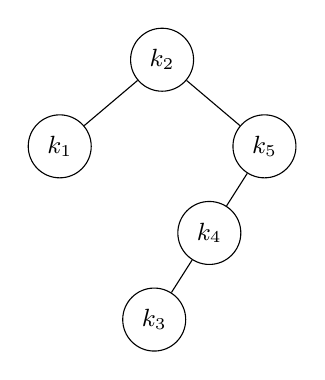
\begin{tikzpicture}[every node/.style={circle,draw,minimum size=8mm,font=\small,inner sep=0pt},
  level distance=11mm, level 1/.style={sibling distance=26mm},
  level 2/.style={sibling distance=14mm}]
\node {$k_2$}
  child {node {$k_1$}}
  child {node {$k_5$}
    child {node {$k_4$}
      child {node {$k_3$}}
      child[missing] {}
    }
    child[missing] {}
  };
\end{tikzpicture}
\\[-1mm]
{\small The optimal BST for the lab instance: heavy keys $k_2,k_5$ ride high.}
\end{center}

\begin{formalbox}
\textbf{Correctness of the optimal-BST recurrence.} We claim $e[i,j]$ as defined
equals the minimum expected cost over all BSTs on keys $k_i,\dots,k_j$. Proof
sketch by induction on the range length $j-i+1$. \emph{Base:} an empty range is
a single dummy leaf $d_{i-1}$ at depth $0$ within the subtree, contributing
$q_{i-1}$; the formula gives exactly that. \emph{Step:} any BST on $k_i,\dots,
k_j$ has \emph{some} root $k_r$; its subtrees are BSTs on $k_i,\dots,k_{r-1}$
and $k_{r+1},\dots,k_j$. By optimal substructure (cut-and-paste), an optimal
overall tree uses optimal subtrees, whose costs are $e[i,r-1]$ and $e[r+1,j]$ by
the induction hypothesis. Rooting at $k_r$ deepens every node of both subtrees
by one, adding $w(i,j)$ to the cost. Minimizing over all valid roots $r$ gives
exactly the recurrence, so the computed $e[i,j]$ is optimal. $\qquad\blacksquare$
\end{formalbox}

\section{Stepping Back: The Shape of a DP}

You have now seen four dynamic programs, and they rhyme. In each, you found a
``last choice'' (first piece, top-level split, last character, root) that broke
the problem into independent optimal subproblems; you wrote a recurrence over a
small, structured space of subproblems; you filled a table in an order
respecting the dependencies; and you stored side information to reconstruct an
actual solution. Internalize that rhythm and most ``hard'' optimization
problems become a matter of \emph{finding the right last choice}.

\begin{complexitybox}
\textbf{Costs at a glance.}
\begin{center}
\begin{tabular}{lccc}
\toprule
Problem & Subproblems & Time & Space \\
\midrule
Rod cutting & $\Theta(n)$ & $\Theta(n^2)$ & $\Theta(n)$ \\
Matrix-chain & $\Theta(n^2)$ & $\Theta(n^3)$ & $\Theta(n^2)$ \\
LCS & $\Theta(mn)$ & $\Theta(mn)$ & $\Theta(mn)$ \\
Optimal BST & $\Theta(n^2)$ & $\Theta(n^3)$ & $\Theta(n^2)$ \\
\bottomrule
\end{tabular}
\end{center}
In every row the time is (number of subproblems) $\times$ (work per subproblem),
where ``work per subproblem'' is the cost of evaluating the $\min$/$\max$ over
all choices.
\end{complexitybox}

\begin{walkbox}
One last walk. Pick any optimization puzzle you have met -- making change with
fewest coins, the longest increasing subsequence of a list, the minimum number
of edits to turn one word into another. For each, ask the three diagnostic
questions: (1) What is the last choice that splits it? (2) Does an optimal
solution force its subparts to be optimal (optimal substructure)? (3) Do the
subproblems overlap? If all three answer yes, you can write the recurrence and
the table on the spot. Try it for ``fewest coins to make $47$ cents with
denominations $\{1,5,10,25\}$'' before you read the exercises.
\end{walkbox}

\section*{Exercises}
\addcontentsline{toc}{section}{Exercises}

\begin{exercise}[Rod cutting by hand]
\label{ch15:ex-rod}
Using the price table of Section~\ref{ch15:rod}, compute $r_9$ and $r_{10}$ by
extending the lab table. For each, give both the maximum revenue and an optimal
list of cuts. (Hint: you already have $r_0$ through $r_8$.)
\end{exercise}

\begin{exercise}[A cheaper-is-better price table]
\label{ch15:ex-rod2}
Suppose every price equals the length: $p_i = i$ for all $i$. Argue that for any
$n$ the optimal revenue is exactly $n$ and that \emph{every} way of cutting is
optimal. What does the choice array $s$ look like, and why does that match your
argument?
\end{exercise}

\begin{exercise}[Memoization order]
\label{ch15:ex-memo}
In \textsc{Memoized-Cut-Rod}, suppose you call it once for $n = 6$. List the
subproblems in the order their final values are \emph{stored} in $r$. How does
this order compare to the bottom-up order $0,1,2,\dots,6$? Explain the
difference in one sentence.
\end{exercise}

\begin{exercise}[Matrix-chain grouping]
\label{ch15:ex-mc}
For the dimension sequence $p = \langle 5, 10, 3, 12, 5, 50, 6\rangle$ (six
matrices), fill the $m$ and $s$ tables and state the optimal cost and
parenthesization. Show at least the length-2 and length-3 diagonals in full.
\end{exercise}

\begin{exercise}[Why not greedy?]
\label{ch15:ex-greedy}
A tempting greedy heuristic for matrix-chain is ``always first multiply the
adjacent pair whose product is cheapest.'' Find a chain of three or four
matrices where this greedy rule produces a \emph{suboptimal} parenthesization,
and explain which DP principle it violates.
\end{exercise}

\begin{exercise}[LCS trace]
\label{ch15:ex-lcs}
Compute an LCS of $X = \texttt{10010101}$ and $Y = \texttt{010110110}$ (treat
each digit as a character). Build the full $c$ table, then read off one LCS by
tracing arrows. State its length.
\end{exercise}

\begin{exercise}[LCS and edit distance]
\label{ch15:ex-edit}
The \emph{edit distance} between two strings is the minimum number of
single-character insertions and deletions (no substitutions) to turn one into
the other. Show that if $X$ and $Y$ have lengths $m$ and $n$ and an LCS of
length $L$, then this edit distance equals $m + n - 2L$. (Hint: characters not
in the common subsequence must be deleted from $X$ or inserted into $Y$.)
\end{exercise}

\begin{exercise}[Counting subsequences]
\label{ch15:ex-count}
Modify the LCS recurrence to instead \emph{count} the number of distinct
longest common subsequences. Write the recurrence for a table $N[i,j]$ that
stores this count alongside $c[i,j]$, being careful about the case
$c[i-1,j] = c[i,j-1]$.
\end{exercise}

\begin{exercise}[Optimal BST sanity check]
\label{ch15:ex-obst}
For the lab instance in Section~\ref{ch15:obst}, verify by hand that the
single-key cost $e[3,3] = 0.25$ is correct: write out $w[3,3]$ and the empty-range
costs it combines, and confirm the arithmetic. Then explain in words why the
optimal tree places $k_2$ (probability $0.10$) at the root rather than the more
probable $k_5$ (probability $0.20$).
\end{exercise}

\begin{exercise}[Balanced is not optimal]
\label{ch15:ex-balanced}
Construct probabilities $p_1, p_2, p_3$ (with all $q_j = 0$) for three keys so
that the optimal BST is a degenerate ``stick'' (each node has at most one child)
rather than the balanced tree with $k_2$ at the root. State your probabilities
and the expected costs of both trees to justify it.
\end{exercise}

\begin{exercise}[Subproblem graph]
\label{ch15:ex-graph}
Draw the subproblem dependency graph for LCS of two length-3 strings (a
$4 \times 4$ grid of nodes $c[i,j]$). Put an edge from each node to every node
it directly depends on. How many edges leave a typical interior node, and how
does that number explain the $\Theta(mn)$ running time?
\end{exercise}

\begin{exercise}[Coins, challenge]
\label{ch15:ex-coins}
Given coin denominations $d_1 < d_2 < \cdots < d_k$ and a target amount $A$,
design a DP that computes the fewest coins summing to exactly $A$ (or reports
impossibility). State the recurrence, the table size, the running time, and how
to reconstruct which coins to use. Then run it for $A = 47$ and denominations
$\{1, 5, 10, 25\}$.
\end{exercise}
